\documentclass[10pt,twocolumn,letterpaper]{article}
\usepackage{tikz}  % For plots, must be the first include

\usepackage{cvpr}
\usepackage{times}
\usepackage{epsfig}
\usepackage{graphicx}
\usepackage{amsmath}
\usepackage{amssymb}

% Include other packages here, before hyperref.
\usepackage{pgfplots} % For plots
\usepackage{pgfplotstable} % For plots
\pgfplotsset{compat=newest} % For plots
\usetikzlibrary{plotmarks} % For plots

% If you comment hyperref and then uncomment it, you should delete
% egpaper.aux before re-running latex.  (Or just hit 'q' on the first latex
% run, let it finish, and you should be clear).
\usepackage[pagebackref=true,breaklinks=true,letterpaper=true,colorlinks,bookmarks=false]{hyperref}

% \cvprfinalcopy % *** Uncomment this line for the final submission

\def\cvprPaperID{752} % *** Enter the CVPR Paper ID here
\def\httilde{\mbox{\tt\raisebox{-.5ex}{\symbol{126}}}}

\usepackage{algorithmic}	% Nice algorithm environment
\usepackage{algorithm}
\newcommand{\todo}[1]{\textbf{\textcolor{red}{[#1]}}}
\newcommand{\dx}[1]{\textbf{\textcolor{green}{[Dengxin:#1]}}}
\newcommand{\yh}[1]{\textbf{\textcolor{blue}{[Yuhua:#1]}}}
\newcommand{\jd}[1]{\textbf{\textcolor{magenta}{[Jordi:#1]}}}
% \newcommand{\etal}{\textit{et al.}}
\usepackage{bbm}

% Pages are numbered in submission mode, and unnumbered in camera-ready
\ifcvprfinal\pagestyle{empty}\fi
\begin{document}

%%%%%%%%% TITLE
\title{Scale-Aware Alignment of Hierarchical Image Segmentation\\ \vspace{0.5cm} Supplementary Material}

\author{First Author\\
Institution1\\
Institution1 address\\
{\tt\small firstauthor@i1.org}
% For a paper whose authors are all at the same institution,
% omit the following lines up until the closing ``}''.
% Additional authors and addresses can be added with ``\and'',
% just like the second author.
% To save space, use either the email address or home page, not both
\and
Second Author\\
Institution2\\
First line of institution2 address\\
{\tt\small secondauthor@i2.org}
}

\maketitle
%\thispagestyle{empty}

%%%%%%%%% ABSTRACT
\section{Training Random Forest With Different Data}

Besides the results reported in the paper, which are based on training a specific Regression Forest (RF) for each segmentation method, we also test training a global RF using segments from all four methods. The experiment settings are similar to previous experiments, only the specific RF in the pipeline is replaced by a global RF. 

Additionally, we also test how well the knowledge learned from one method generalizes to other methods. Since we gain the most improvement by the RF trained by MCG segments, we apply the RF trained by MCG segments to other three methods, while keep other conditions unchanged.

All results are summarized in Table~\ref{tab:detail_res}. Entries with '+specific RF' represent results using specific RF (the results reported in our paper). Entries with '+global RF' and '+MCG RF' stand for results of RF trained by all the segments and MCG segments, respectively. As it can be seen in Table~\ref{tab:detail_res}, the specific RFs give the best results. The results in the other tested scenarios are slightly worse than the specific one, but they still improve the original MCG hierarchies.
%The results  suggest that segments produced by different methods have different traits, thus we can take advantage of it to achieve better results by training a specific RF. 

\begin{table}
\begin{center}
\resizebox{0.5\textwidth}{!}{
\begin{tabular} {| c | c | c | c | c | c | c |}
\hline
& \multicolumn{2}{c|}{Covering ($\uparrow$)} & \multicolumn{2}{c|}{PRI ($\uparrow$)} 
& \multicolumn{2}{c|}{VI ($\downarrow$)} \\ \cline{2-7}
 & ODS & OIS & ODS & OIS & ODS & OIS \\ \hline
MCG &
0.611  & 0.672  & 0.832  & 0.861  & 1.570  & 1.390  \\
MCG+specific RF   &
0.626  & 0.679  & 0.832  & 0.862  & 1.525  & 1.378  \\
MCG+global RF   &
0.622  & 0.674  & 0.831  & 0.861  & 1.541  & 1.387  \\ 
\hline
SCG &
0.600  & 0.659  & 0.829  & 0.860  & 1.628  & 1.422  \\ 
SCG+specific RF  &
0.612  & 0.671  & 0.833  & 0.861  & 1.586  & 1.410  \\ 
SCG+global RF  &
0.612  & 0.667  & 0.830  & 0.860  & 1.582  & 1.415  \\ 
SCG+MCG RF  &
0.608  & 0.669  & 0.832  & 0.860  & 1.606  & 1.413  \\ 
\hline
gpb &
0.594  & 0.653  & 0.827  & 0.856  & 1.690  & 1.475  \\ 
gpb+specific RF  &
0.608  & 0.663  & 0.828  & 0.858  & 1.642  & 1.460  \\ 
gpb+global RF   &
0.606  & 0.661  & 0.827  & 0.857  & 1.645  & 1.466  \\ 
gpb+MCG RF  &
0.603  & 0.660  & 0.828  & 0.857  & 1.659  & 1.465  \\ 
\hline
PMI &
0.533  & 0.585  & 0.760  & 0.813  & 2.025  & 1.822 \\ 
PMI+specific RF  &
0.543  & 0.590  & 0.760  & 0.815  & 1.996  & 1.813 \\ 
PMI+global RF  &
0.540  & 0.588  & 0.760  & 0.814  & 2.006  & 1.810  \\
PMI+MCG RF   &
0.539  & 0.589  & 0.759  & 0.814  & 2.008  & 1.815 \\ 
\hline
\end{tabular}}
\end{center}
\caption{Benchmark results on BSDS500 test set. '+specific RF', '+global RF' and '+MCG RF' represent results trained by specific segments, all the segments and MCG segments, respectively.}
\label{tab:detail_res}
\end{table}

\section{Regressing Covering}
As mentioned in the paper, a key difference between our prediction and some previous
works is that they predict the quality of segments (overlap with ground truth), while we
predict their scale.
Instead of only knowing whether a segment is good or not, we aim to predict its scale,
which makes our prediction more informative.
To test if the extra information is helpful to the task of aligning hierarchy,
we train a RF only to predict the segmentation quality.
In this scenario, we use the Intersection over Union (IoU) as the quality, like to many previous works.
Formally, the quality of a segment \textbf{s} is defined as:
\begin{equation}
 q(\textbf{s}) = \max_{\textbf{g}}\frac{|\textbf{s}\cap\textbf{g}|}{|\textbf{s}\cup\textbf{g}|}
\end{equation}
where $\textbf{g}$ are the fragments in the ground truth.
We extract training segments and train a regression forest to predict their IoU.
To find anchor slice in this case, we use a similar formulation using only predicted quality:

\begin{equation}
  \label{eq:energy}
  \begin{split}
    &\hat{\mathbf{X}} = arg\min_{\mathbf{X}} E(\mathbf{X})\\
 E(\mathbf{X})& =  - \sum_{v_i \in \mathcal{L}} \#(v_i) \cdot q(v_i) \\
 \text{s.t   }  \quad \forall n: & \quad \sum_{v \in \mathcal{P}_n} \mathbbm{1}_\mathcal{L} (v) = 1\\
              \quad \forall v:  & \quad x(v) >= x(v^p)\\
   \end{split}
\end{equation}
In the above equation, $\#(v)$ is the size (number of pixels) of segment (node) $v$.
Compared to the original formulation, the energy term is replaced into segmentation quality.
All the constraints remain unchanged. Again, Eq~\ref{eq:energy} is solvable via dynamic programming.

We test the new formulation on the BSDS500 dataset, using the same experimental settings.
As the results show in Table~\ref{tab:res_baseline}, the performance of the new baseline is much worse
than the original one.
The margin validates the usefulness of predicting the scale.
%We argue that predicting scale is more reliable than quality, since prediction based on mid-level features is noisy and the extra information can provide some regularization to improve performance. 

\begin{table}
\begin{center}
\resizebox{0.5\textwidth}{!}{
\begin{tabular} {| c | c | c | c | c | c | c |}
\hline
& \multicolumn{2}{c|}{Covering ($\uparrow$)} & \multicolumn{2}{c|}{PRI ($\uparrow$)} 
& \multicolumn{2}{c|}{VI ($\downarrow$)} \\ \cline{2-7}
 & ODS & OIS & ODS & OIS & ODS & OIS \\ \hline
MCG &
0.611  & 0.672  & 0.832  & 0.861  & 1.570  & 1.390  \\
MCG-aligned by scale &
0.626  & 0.679  & 0.832  & 0.862  & 1.525  & 1.378  \\
MCG-aligned by quality &
0.615  & 0.673  & 0.831  & 0.859  & 1.562  & 1.385 \\
\hline
\end{tabular}}
\end{center}
\caption{Benchmark results of two different formulations.}
\label{tab:res_baseline}
\end{table}

\section{Visual Results of Other Hierarchies}
Due to the limit of space, only visual results of MCG hierarchies are included in our paper. Following we include some results of SCG and gpb hierarchies in Fig~\ref{fig:more_hier}.
Similar to MCG hierarchies, our approach shows a consistent improvement and provide better alignment over the original hierarchies. 

\begin{figure*}
\begin{center}
\begin{tabular}{c}
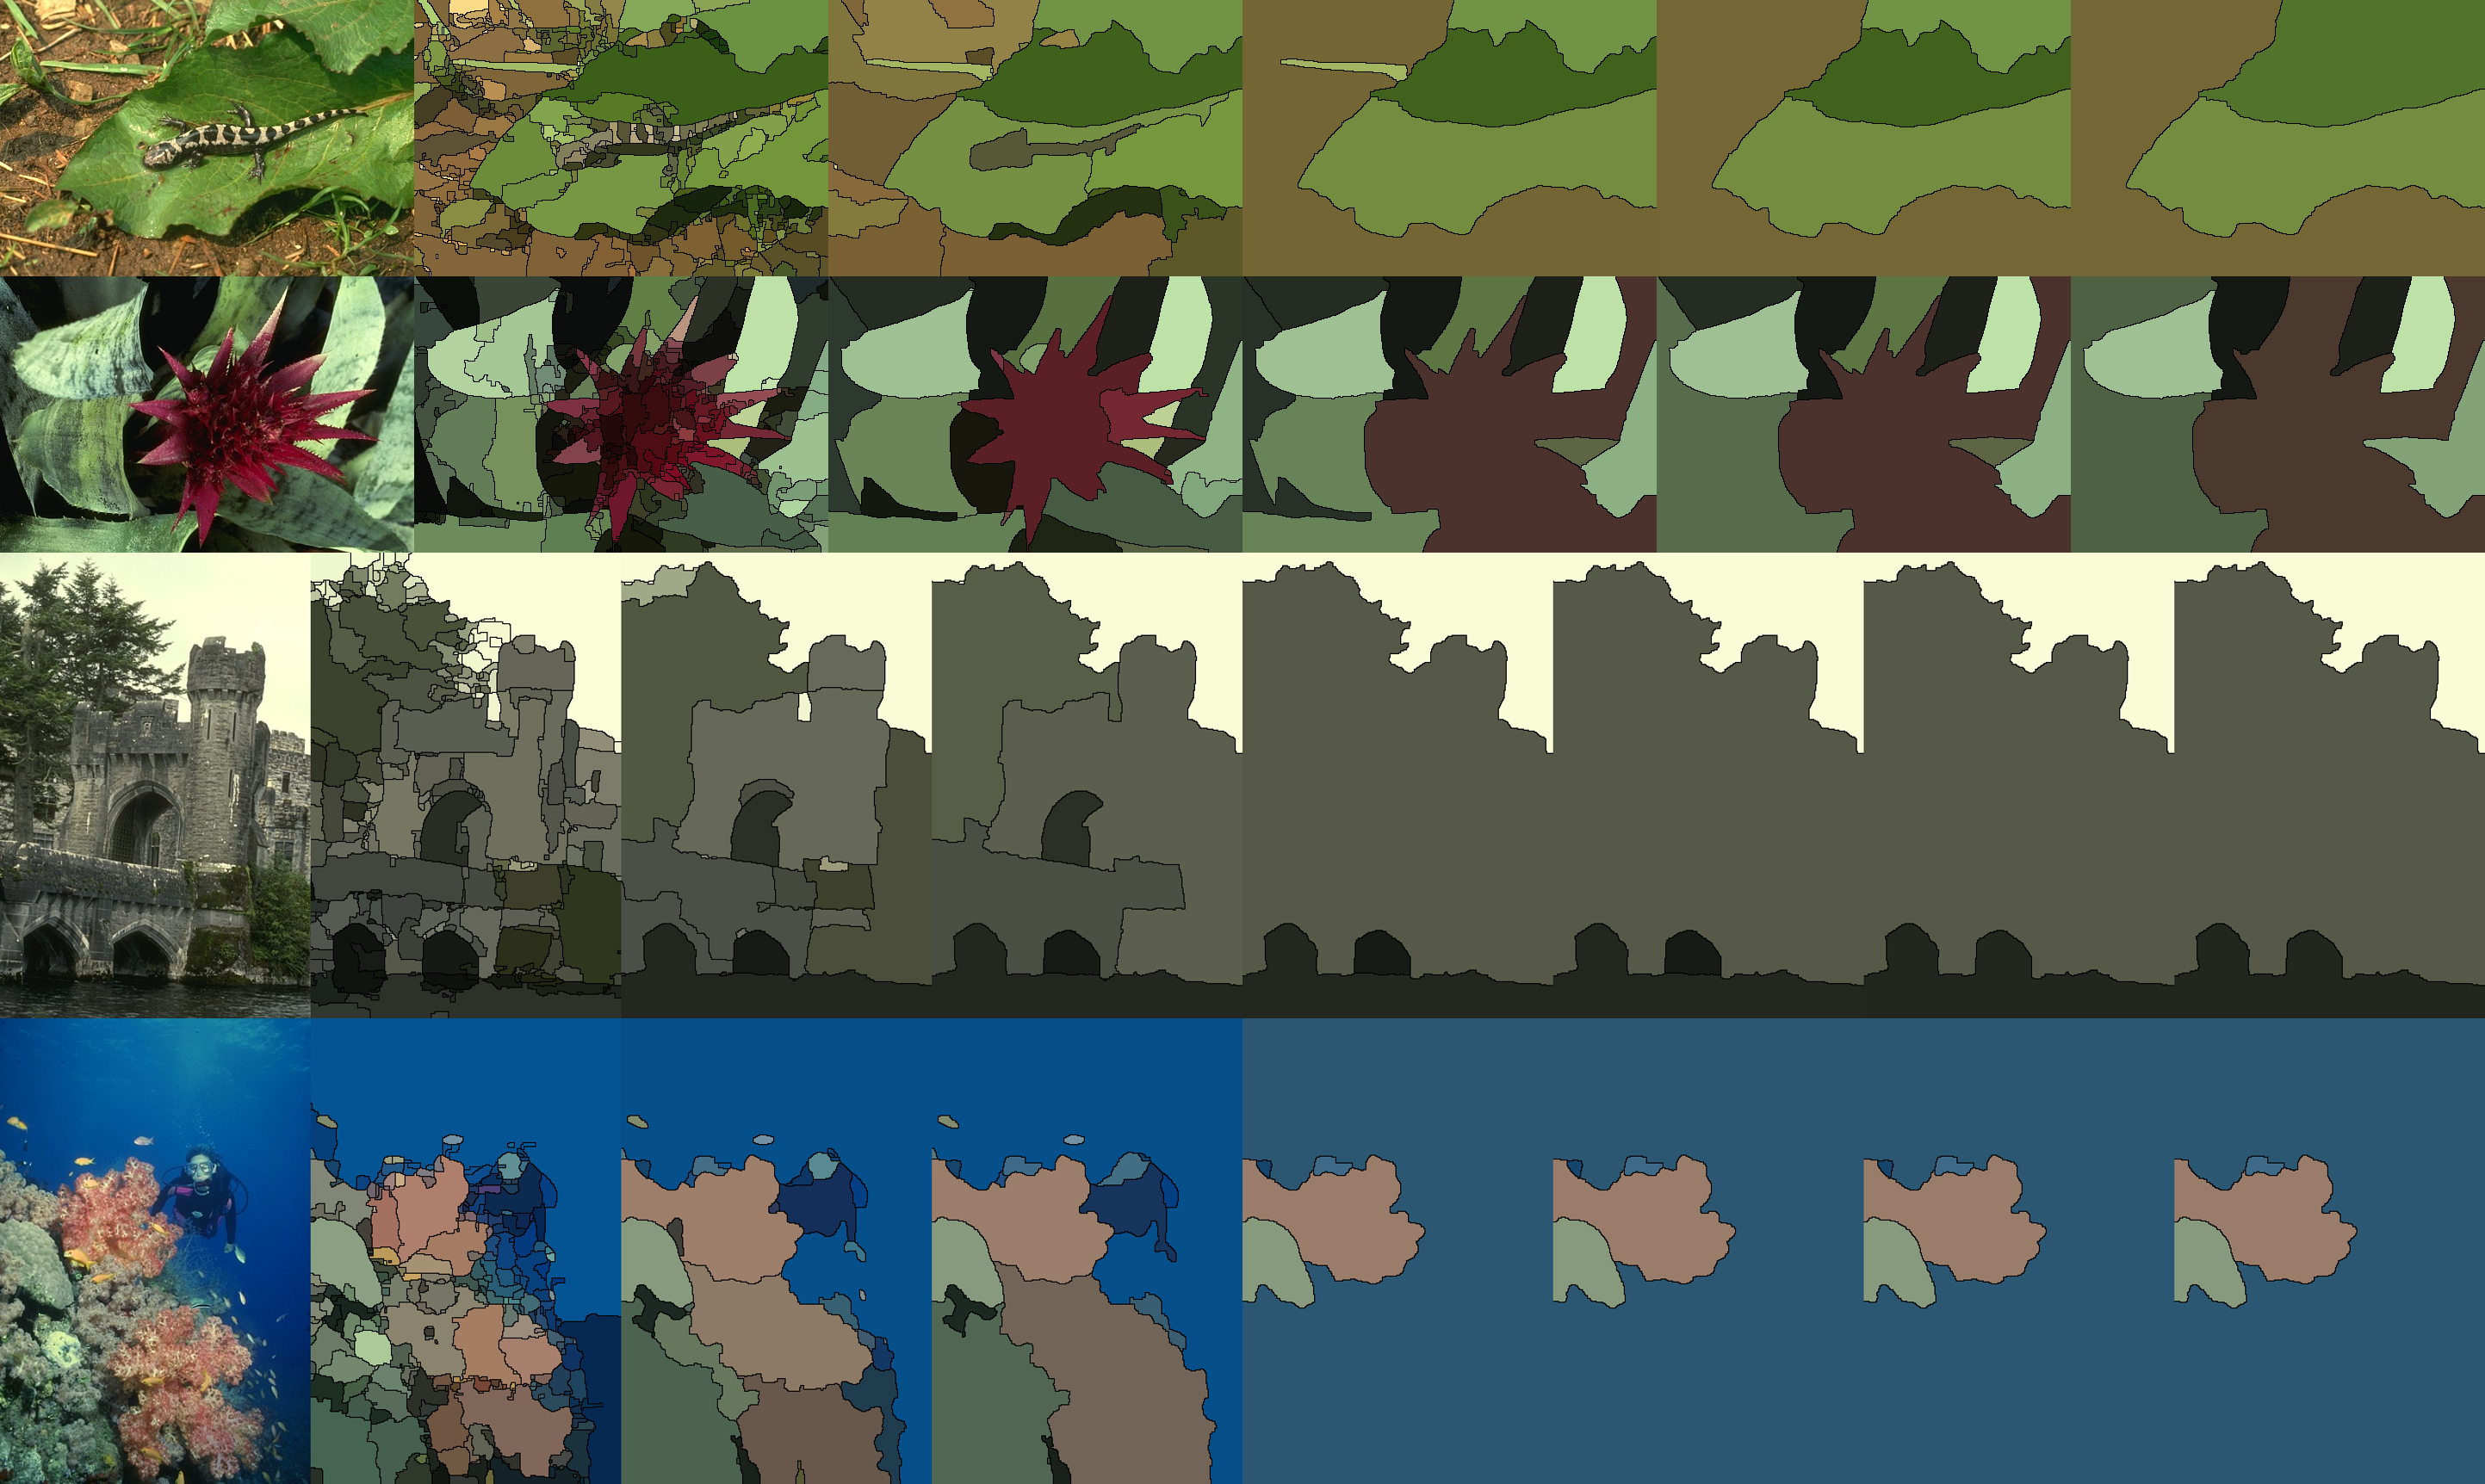
\includegraphics[width=17cm]{fig/smfig/stack_scg.png} \\
SCG\\ \\
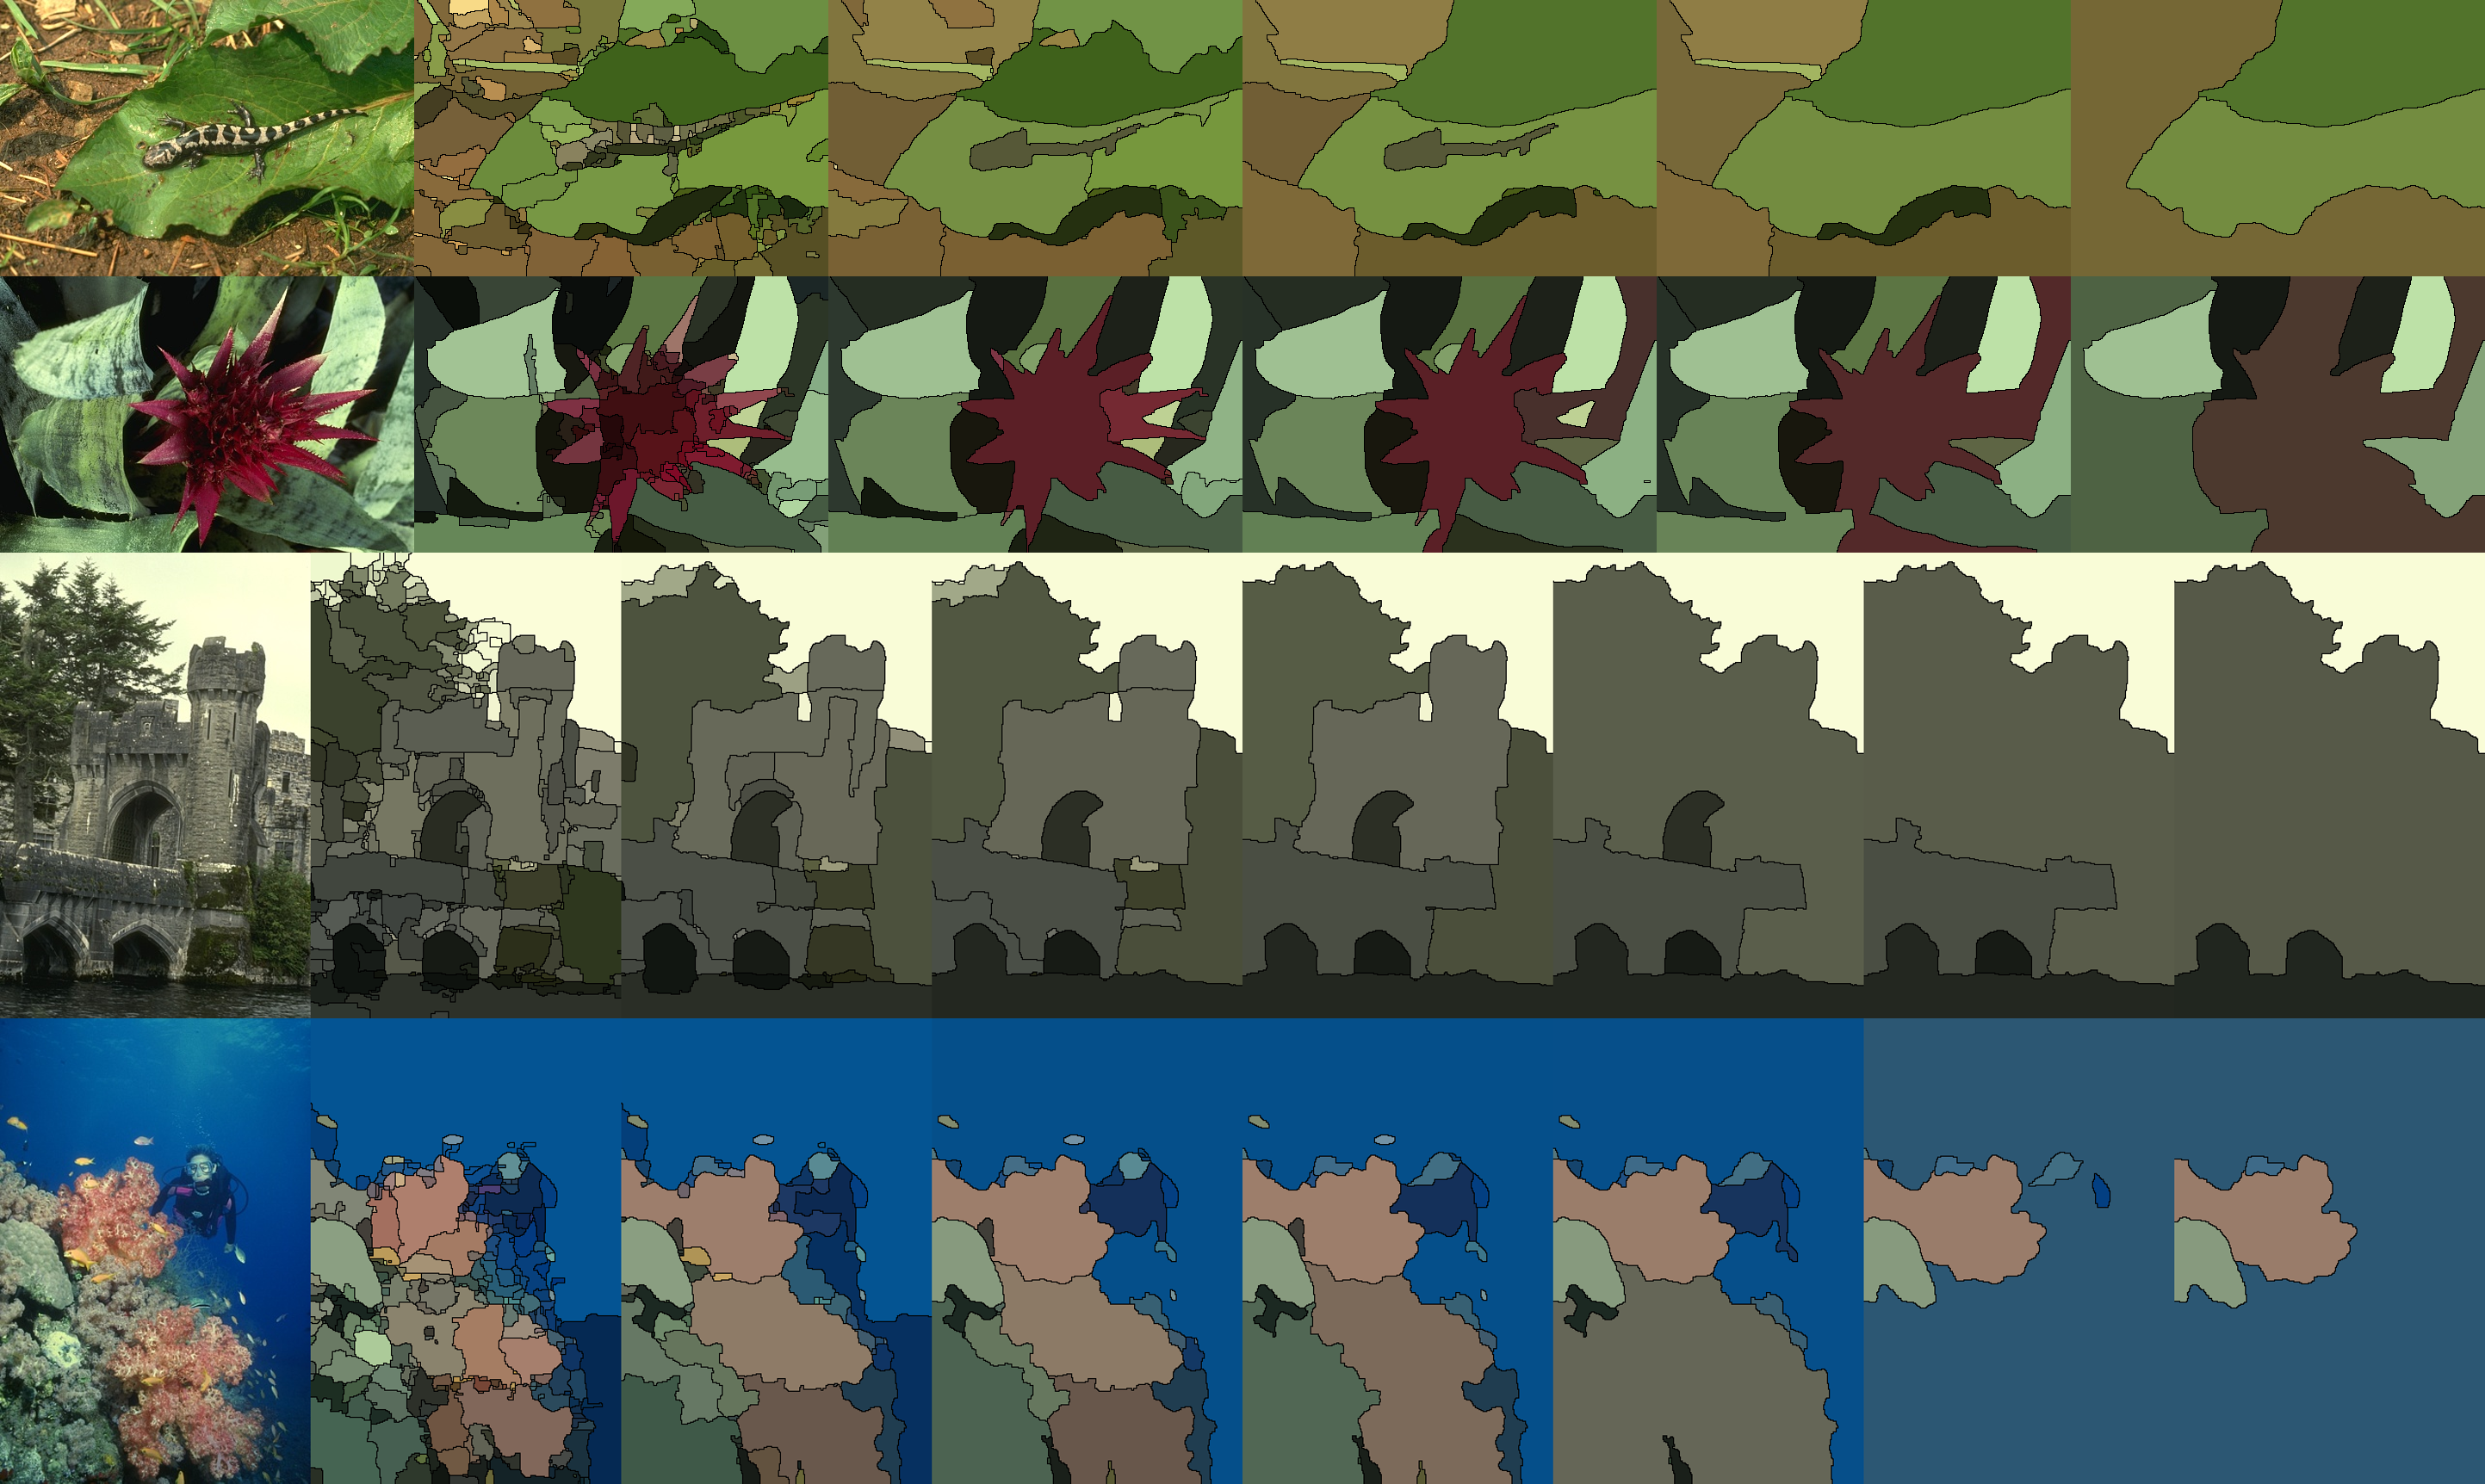
\includegraphics[width=17cm]{fig/smfig/stack_scg_a.png}\\
SCG-aligned\\
\end{tabular}
\end{center}
\end{figure*}

\begin{figure*}[tb]
\begin{center}
\begin{tabular}{c}
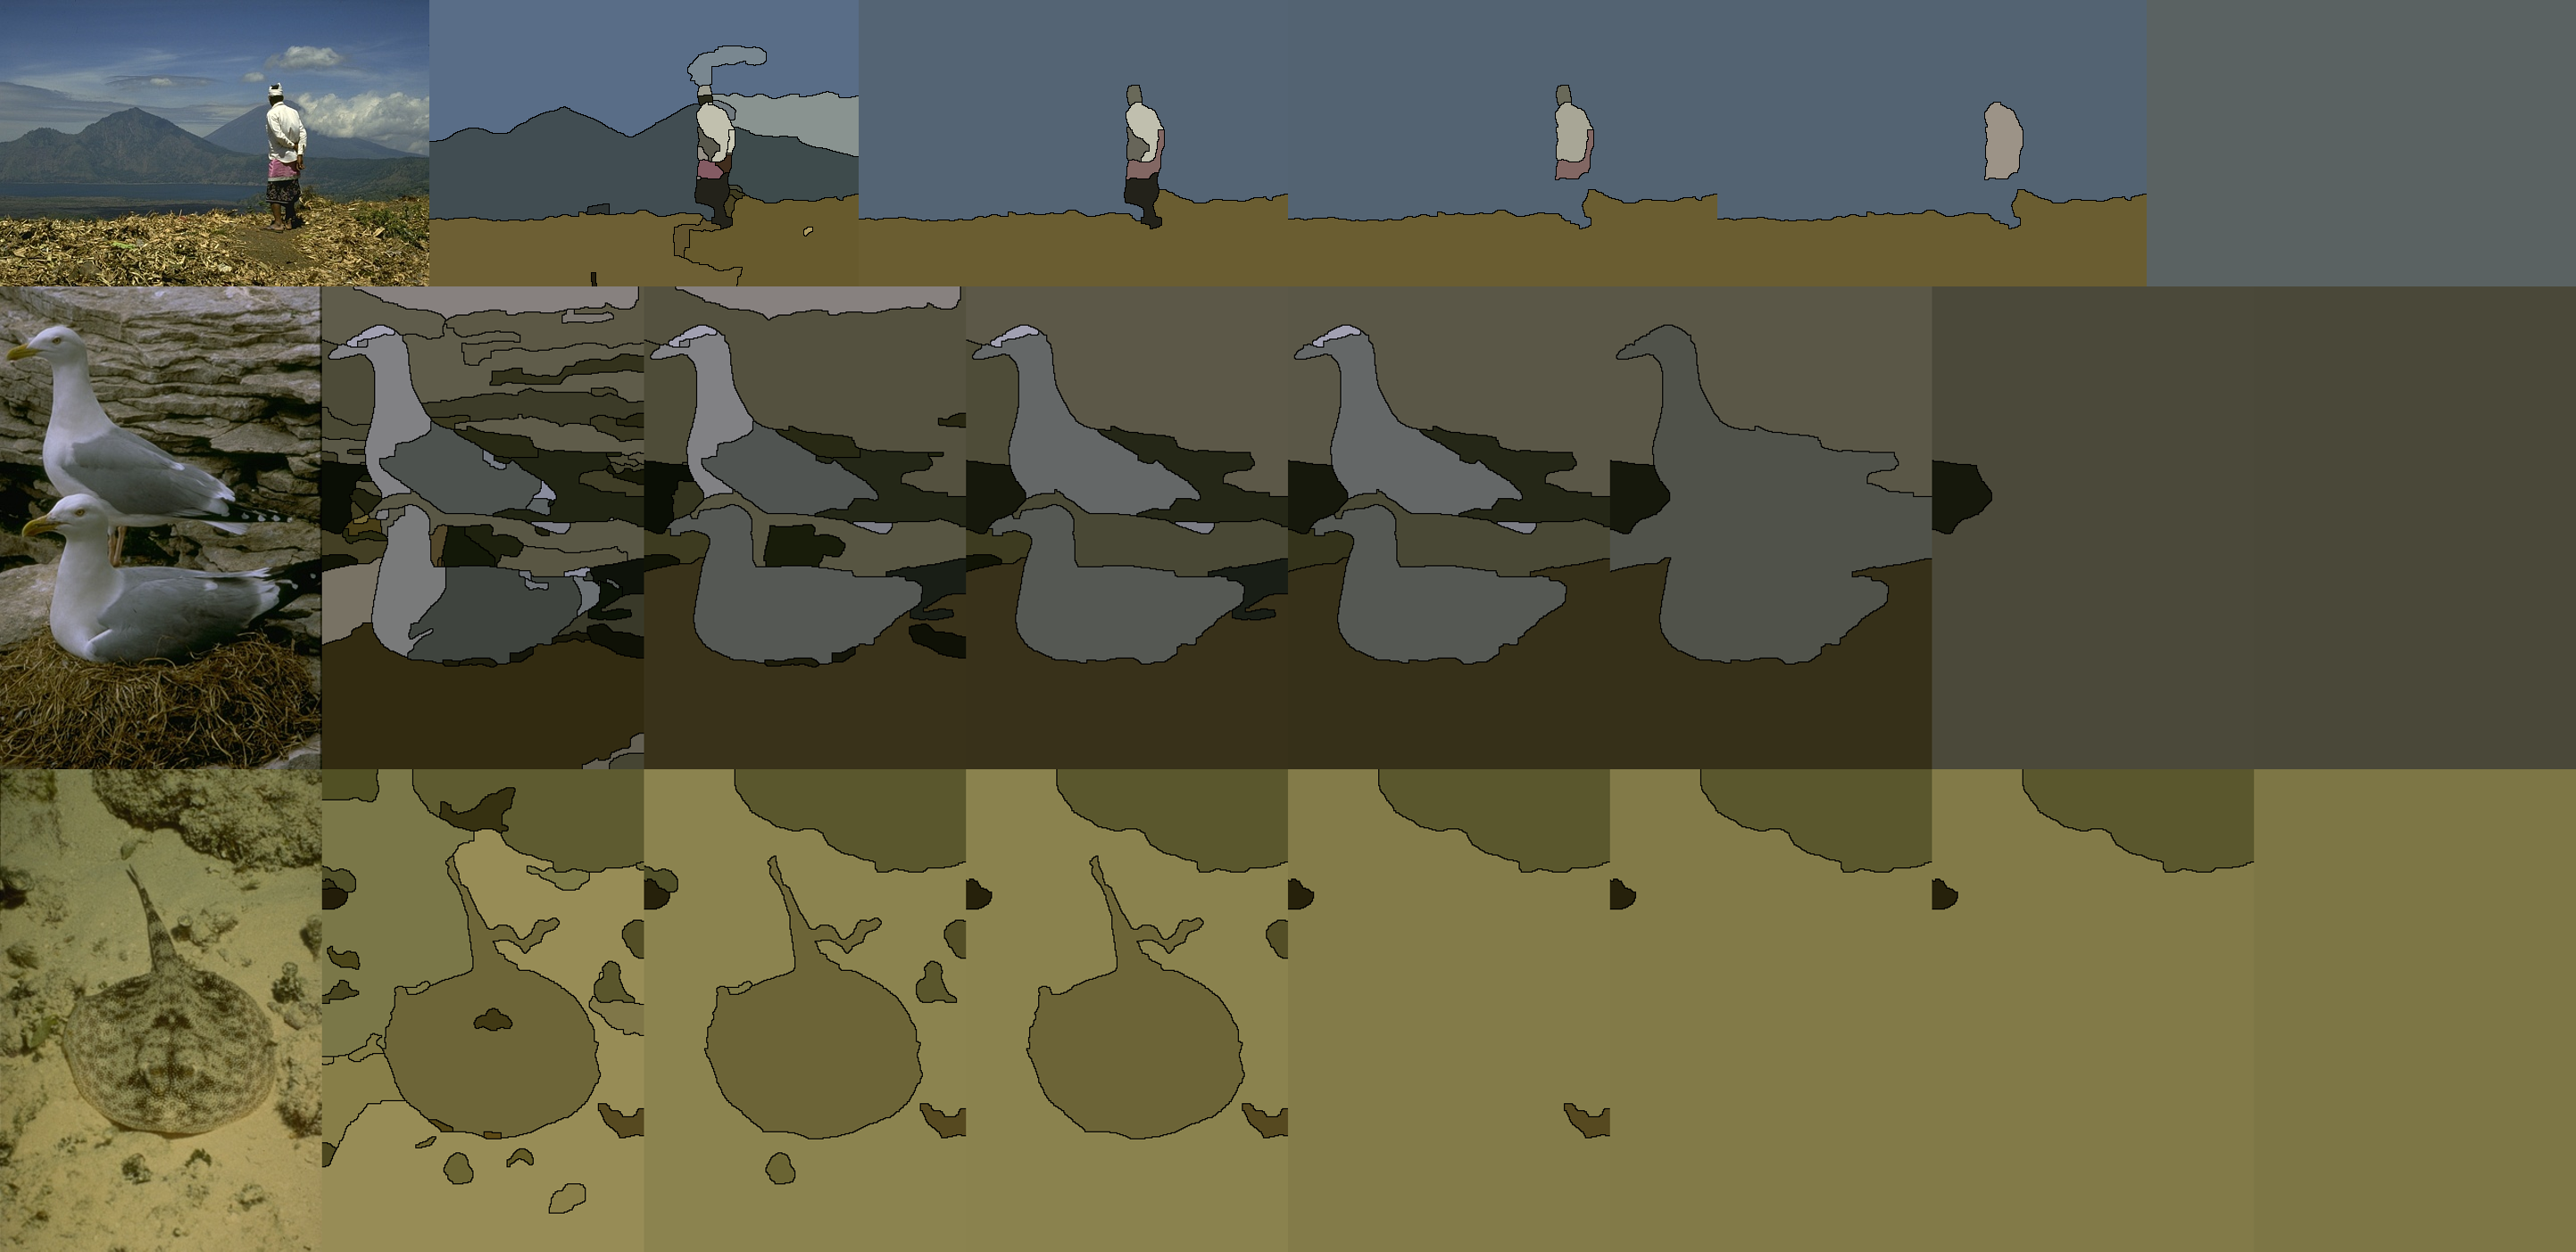
\includegraphics[width=17cm]{fig/smfig/stack_gpb.png} \\
gpb\\ \\
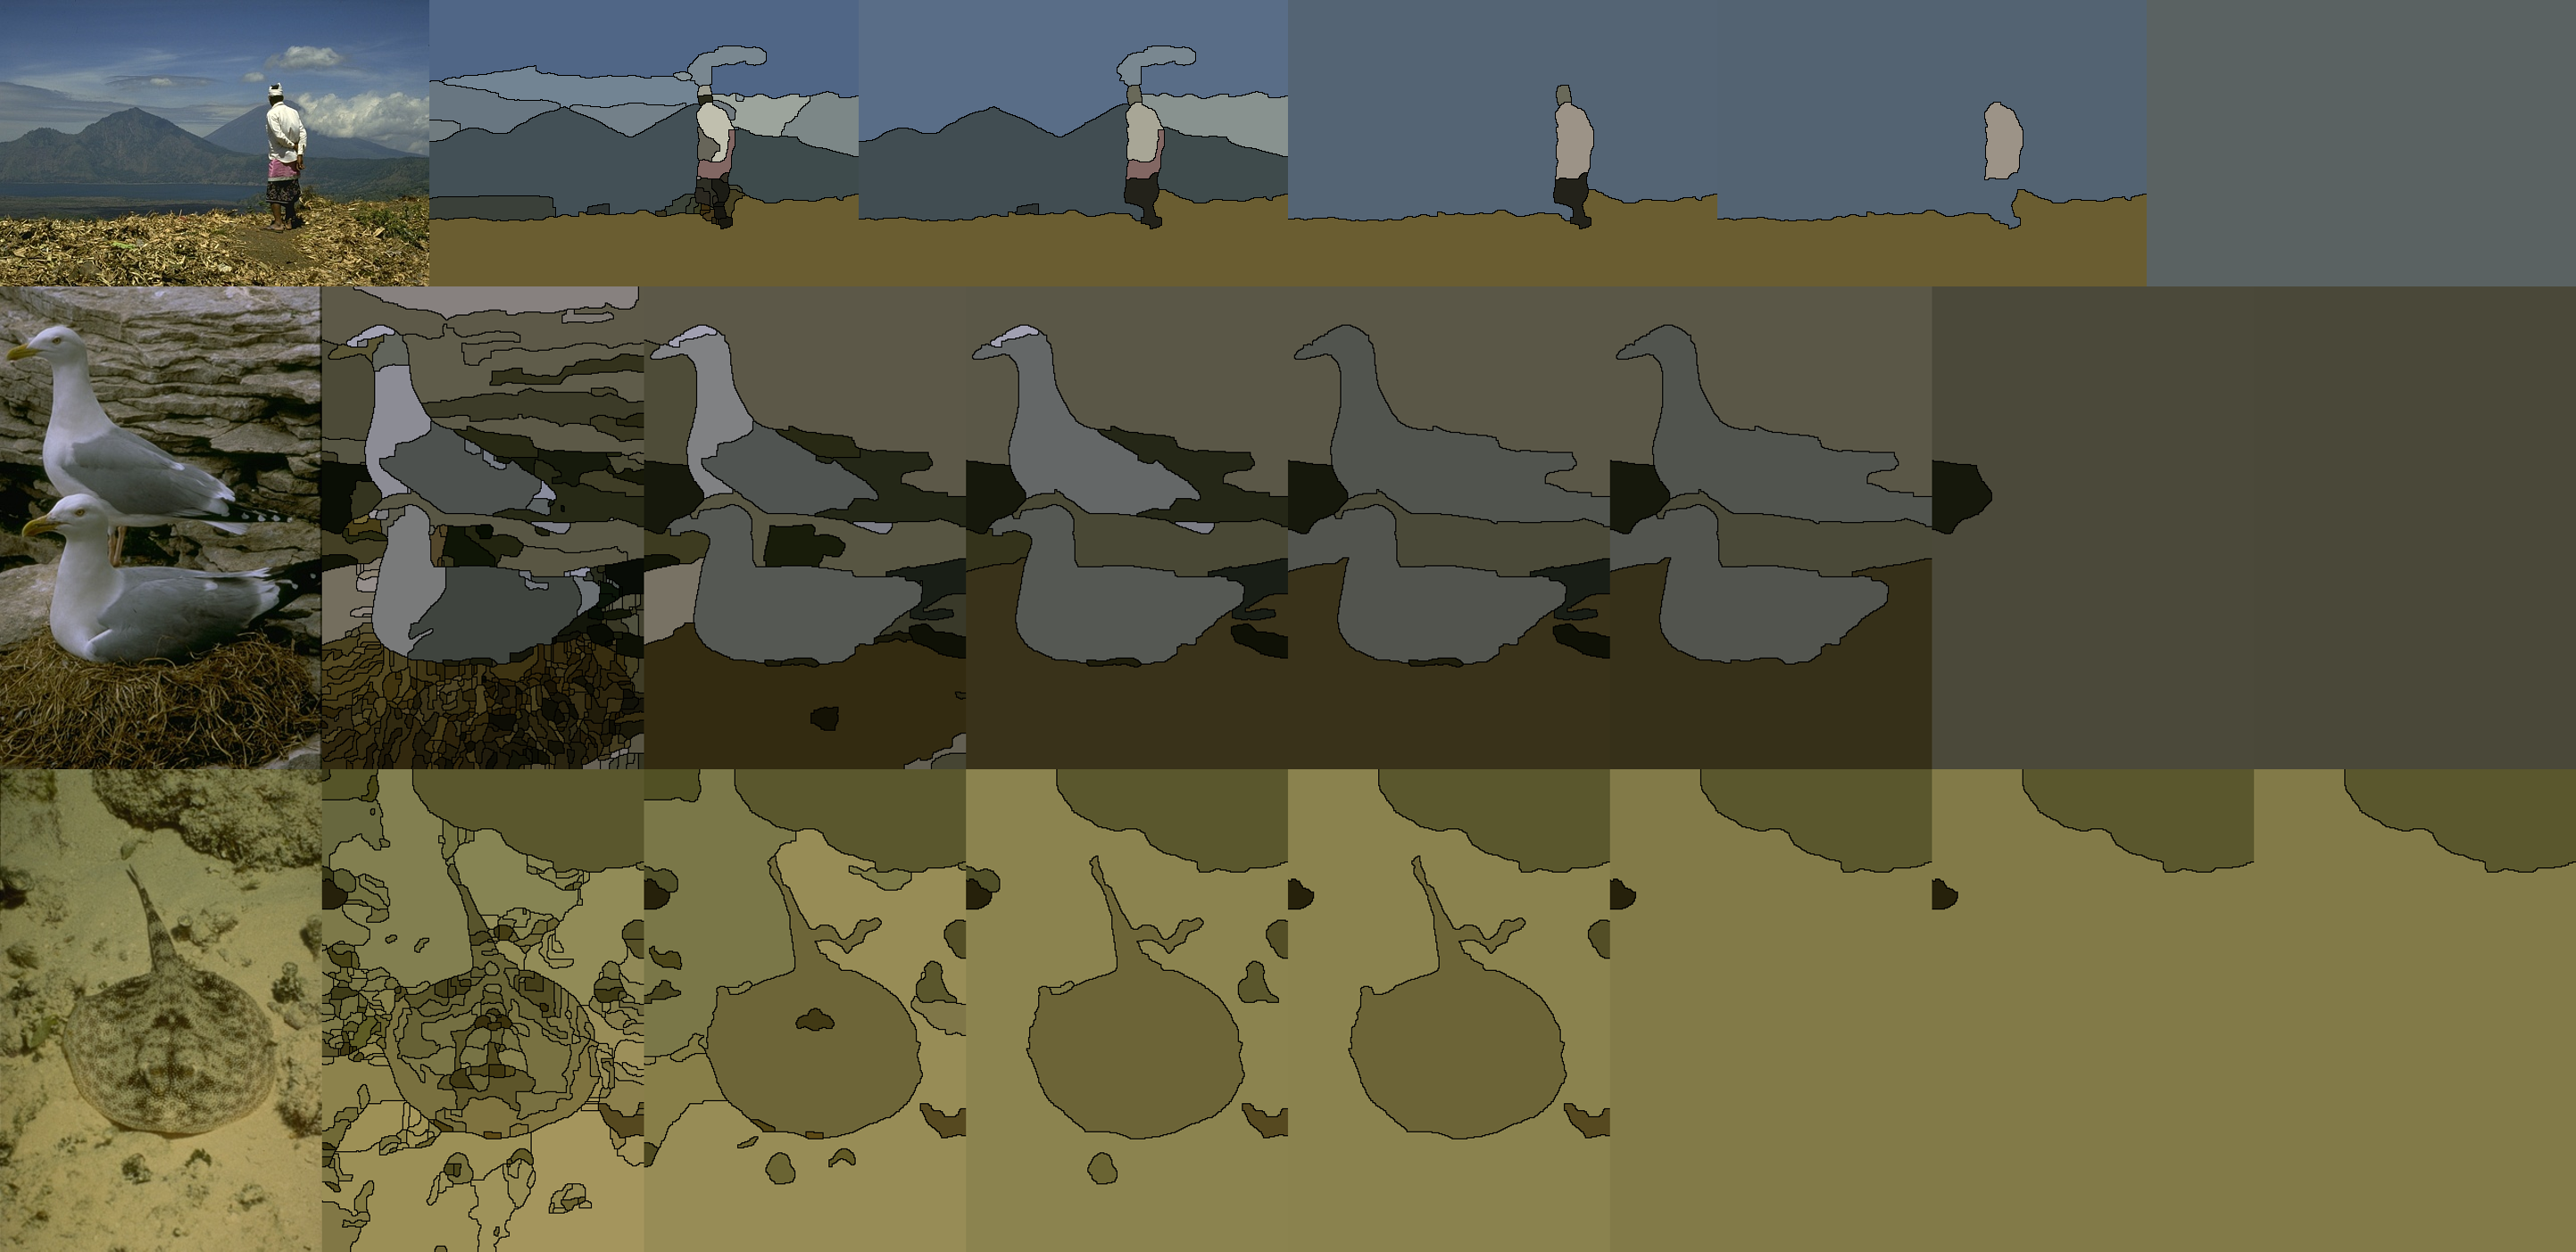
\includegraphics[width=17cm]{fig/smfig/stack_gpb_a.png} \\
gpb-aligned
\end{tabular}
\end{center}
\caption{Results of other hierarchies. From top to bottom: SCG, SCG-aligned, gpb, gpb-aligned. Original images are shown in the left most. For each method, segmentations of optimal-dataset-sclae(ODS) are shown in the middle. And from left to right are different scales, from fine to coarse.}
\label{fig:more_hier}
\end{figure*}





\end{document}
